\chapter{Scheduling}
In contemporary operating systems, it is common to have many programs in memory, executing concurrently. To give the illusion of multiple programs running `at the same time' on a single core, program execution is interleaved, by letting a program run for a small time slice before switching to another. Many different algorithms for deciding what program to run at a given time are available, optimizing for different system characteristics.

\section{The scheduling problem}
\textcite{buttazzo2011hard} defines the scheduling problem as follows. Given a set of $n$ tasks $\Gamma = \set{\tau_1, \tau_2, \ldots, \tau_n}$, a set of $m$ processors $P = \set{P_1, P_2, \ldots, P_m}$, a set of $s$ types of resources $R = \set{R_1, R_2, \ldots, R_s}$, a directed acyclic graph (DAG) describing the precedence relation among tasks, and a set of timing constraints associated with each task, assign processors from $P$ and resources from $R$ to tasks in $\Gamma$ in order to complete all tasks under the specified constraints. The scheduling problem, in its general form, has been shown to be NP-complete, and hence computationally intractable.

Despite this general intractability, many algorithms have been developed which solve a more specific version of the scheduling problem. These scheduling algorithms have some common characteristics, which are outlined below.

\section{Characteristics of scheduling algorithms}
The following scheduling algorithm classes are adapted from \textcite{buttazzo2011hard}:
\begin{outline}
    \1 Preemptive vs. Non-preemptive
        \2 In preemptive schedulers, a running task can be interrupted at any time and switched out for another task.
        \2 In non-preemptive algorithms, a task is executed until completion.
    \1 Static vs. Dynamic
        \2 In static (or fixed-priority) schedulers, scheduling decisions are taken based on parameters that do not change as the system is running. In dynamic schedulers, these parameters can change during system evolution.
    \1 Guarantee-backed vs. Best-effort
        \2 In a guarantee-backed scheduling algorithm, tasks are only accepted if a guarantee can be made that they can be scheduled, whereas in a best-effort system, tasks may be accepted that cannot be allowed to run to completion for fear of jeopardizing other tasks.
\end{outline}

\noindent In this thesis, the focus lies on preemptive, guarantee-backed schedulers.

\section{Task characteristics in real-time systems}
Scheduling algorithms usually make decisions on which task to schedule based on characteristics of the tasks in the given task set, perhaps augmented with characteristics of the system they are running on. A few task characteristics that are common on real-time systems, and used in the scheduling algorithms below, are detailed below. An illustration of these characteristics can be seen in figure~\ref{fig:taskcharacteristics}.

\begin{figure}[htpb]
    \centering
    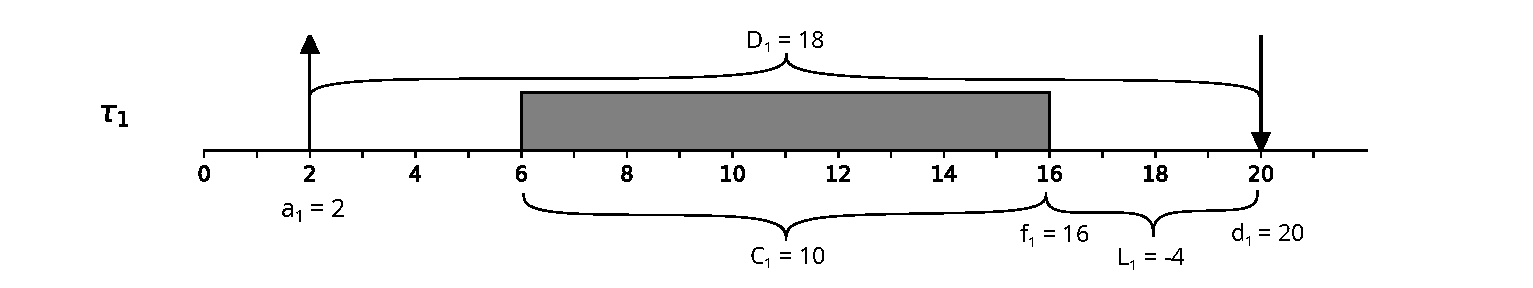
\includegraphics[width=\textwidth]{figures/taskcharacteristics.eps}
    \caption{An overview of common real-time task characteristics.}
    \label{fig:taskcharacteristics}
\end{figure}

\begin{outline}
    \1 A task's \textbf{arrival time} ($a_i$) (also called \textbf{release time} $r_i$) is the time at which a task becomes ready for execution;
    \1 A task's \textbf{computation time} ($C_i$) is the time necessary for the processor to execute the task, without interruption;
    \1 A task's \textbf{absolute deadline} ($d_i$) is the time before which a task should be completed to avoid damage to the system;
    \1 A task's \textbf{relative deadline} ($D_i$) is the difference between the task's arrival time and its absolute deadline: $D_i = d_i - a_i$;
    \1 A task's \textbf{finishing time} ($f_i$) is the time at which a task finishes execution;
    \1 A task's \textbf{lateness} ($L_i$) is the difference between the task's absolute deadline and its finishing time.
\end{outline}

\noindent This thesis focuses on periodic task sets, where each task consists of an infinite number of task instances which are run periodically. The period for a given periodic task is denoted $T_i$. The task characteristics above can vary per instance; all instances will have the same relative deadline, but the absolute deadline obviously varies. To refer to a characteristic for a specific instance, the notation $d_{i,k}$ is commonly used, where we refer to the absolute deadline of the $k$th instance of task $\tau_i$. Furthermore, periodic task sets have a \emph{hyperperiod}, denoted $H$, which is the period after which the entire task set schedule repeats itself. In the case of a periodic task set with relative deadlines equal to or smaller than periods, the hyperperiod is simply equal to the least common multiple of all periods in a task set; i.e.

\begin{equation}
    H = \lcm(T_1, T_2, \ldots, T_n)
\end{equation}

Commonly, a periodic task's relative deadline is equal to its period. In the following figures in this thesis, since arrival times and deadlines coincide, they are shown simply as vertical lines, instead of as arrows.

\section{Fixed-priority scheduling: Rate Monotonic}
The \emph{Rate Monotonic} algorithm is a scheduling algorithm for periodic task sets which assigns priorities based on the frequency of the task, where, if the task needs to run more often, it gets a higher priority. Rate Monotonic is a fixed-priority assignment, so task priorities do not change over time. \textcite{Liu1973} proved the optimality of Rate Monotonic among fixed-priority assignments.

An example task set as scheduled by Rate Monotonic can be seen in figure~\ref{fig:rmexample}. As $\tau_1$ has a smaller period, it has higher priority than $\tau_2$.

\begin{figure}[htpb]
    \centering
    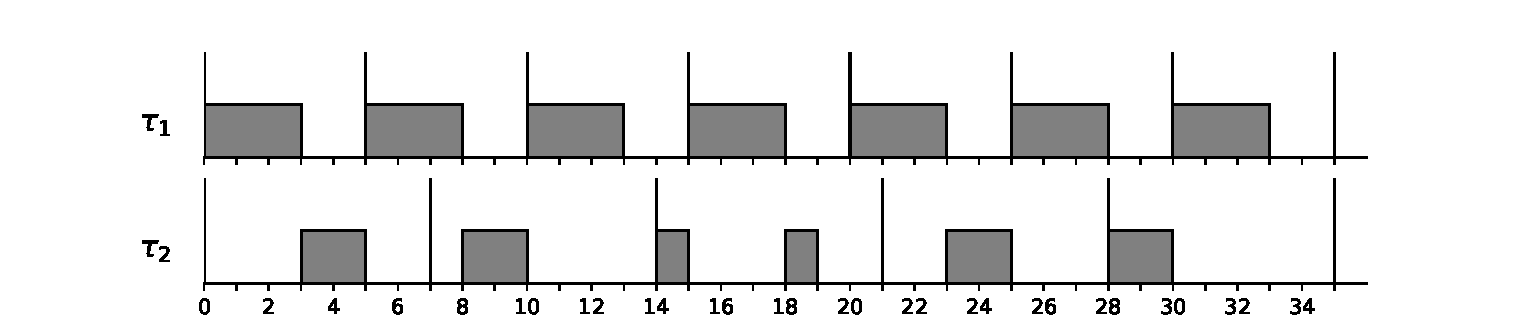
\includegraphics[width=0.9\textwidth]{figures/rmexample.eps}
    \caption{An example task set as scheduled by the Rate Monotonic algorithm.}
    \label{fig:rmexample}
\end{figure}

\section{Dynamic-priority scheduling: Earliest Deadline First}
The \emph{Earliest Deadline First} algorithm is a solution to the problem of scheduling $n$ independent tasks on a uniprocessor system, with dynamic arrivals and preemption. The algorithm simply picks the task with the earliest absolute deadline among all ready tasks, and executes it. When a new task arrives with an earlier deadline, the running task is preempted in favor of the new task.

The Earliest Deadline First algorithm is optimal with respect to maximum lateness; i.e. it minimizes the maximum lateness of tasks in a task set. Due to its dynamic priority assignment, it can achieve a greater processor utilization than fixed-priority assignments such as Rate Monotonic. One example of EDF producing a feasible schedule where RM does not can be seen in figure~\ref{fig:edfrmfeasible}.

\begin{figure}[htpb]
    \centering
    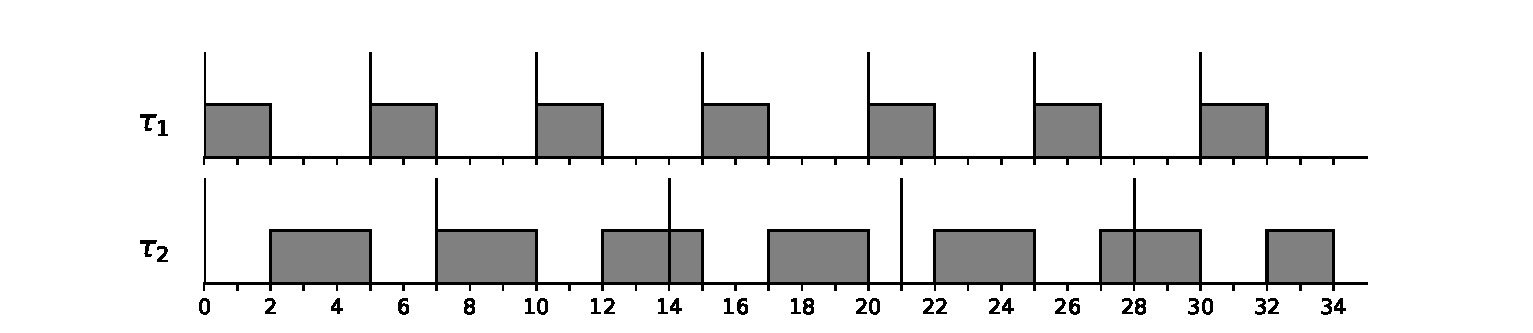
\includegraphics[width=0.9\textwidth]{figures/rmfail.eps}
    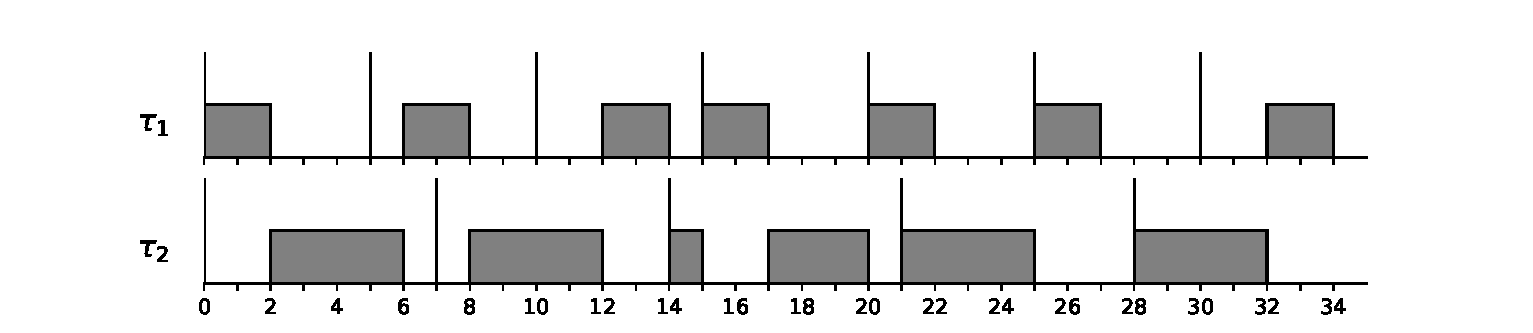
\includegraphics[width=0.9\textwidth]{figures/edfsucc.eps}
    \caption{A comparison of schedules generated for a task set with $\tau_1 = (C = 2, T = 5)$ and $\tau_2 = (C = 4, T = 7)$. Above, the Rate Monotonic schedule can be seen to miss a deadline for the first instance of $\tau_2$, whereas EDF produces a feasible schedule for the task set.}
    \label{fig:edfrmfeasible}
\end{figure}

In its elementary form, EDF is incapable of handling task sets which have resource or precedence constraints. Extensions to EDF have been developed which take these extra constraints into account; one of them, which handles precedence constraints, is described below.

\subsubsection{Precedence constraints}
Using a transformation on the task set, EDF can be extended to handle dependent tasks\cite{Chetto1990}. The idea is as follows. Say we have a task set, with two tasks: \task{1} and \task{2}, where \task{2} is dependent on \task{1}. To honor this precedence constraint, we can modify the arrival time of \task{2}, so that it cannot start before \task{1} has finished. Note that, if there is a valid schedule for the task set which satisfies the precedence constraint, the following conditions are met:

\begin{align}
    s_2 \ge a_2 \quad &\text{(\task{2} cannot start before its arrival time)}\\
    s_2 \ge a_1 + C_1 \quad &\text{(\task{2} cannot start before the minimum finishing time of \task{1})}
\end{align}

To guarantee both of these, we can set $s_2$ equal to $\max(a_2, a_1 + C_1)$.

Similarly, task deadlines need to be modified, so that \task{1} finishes before the last possible start time of \task{2}, that being $d_2 - C_2$.

\section{Schedulability analysis}
The task sets that can be scheduled vary by scheduling algorithm, although there are of course task sets which are not schedulable by even a clairvoyant scheduling algorithm. We would like to evaluate whether task sets are schedulable before running them in a system, as to prevent situations where tasks miss their deadlines. This is commonly called \emph{schedulability analysis}.

\subsection{Processor utilization}
There are a number of metrics that tell us something about the required computation time for a given periodic task set. One such metric is the $U$, the \emph{processor utilization} of a task set -- the fraction of processor time required by the task set. This is given by

\begin{equation}
U = \sum_i \dfrac{C_i}{T_i}
\end{equation}

This provides a simple necessary criterion for task sets to be schedulable: $U \le 1$. If the processor utilization is above one, the required computation time exceeds the available processor time, and so the task set is not schedulable by any algorithm.

\subsection{Rate Monotonic}
\textcite{Liu1973}, after describing the Rate Monotonic scheduling algorithm, and proving its optimality among fixed-priority scheduling algorithms, analyzes its least upper bound on processor utilization, under the assumption that the relative deadline of a task is equal to its period. In short, the least upper bound determines the maximum processor utilization under which task sets are always schedulable by the Rate Monotonic algorithm. The least upper bound varies by the number of scheduled tasks; for $m$ tasks, Liu and Layland determine it to be equal to

\begin{equation}
U_{\text{lub}} = m(2^{1/m} - 1)
\end{equation}

\noindent which tends to $\ln 2 \approx 0.69$ as $m$ goes to infinity.

The mathematics behind the derivation is not too complicated, but explaining the derivation in detail could easily take up five pages; therefore, I'll simply refer to the thorough explanation in \textcite[pp. 90-97]{buttazzo2011hard}.

One interesting note is the variance of the upper bound depending on the ratio between task periods. Specifically, when, for each pair of tasks, their period is harmonically related\cite[\S 4]{Buttazzo2005}, the upper bound is equal to 1. As an illustration, for two tasks, the upper bound on processor utilization for varying $T_1 / T_2$ can be seen in figure~\ref{fig:ubk}.

\begin{figure}[htpb]
    \centering
    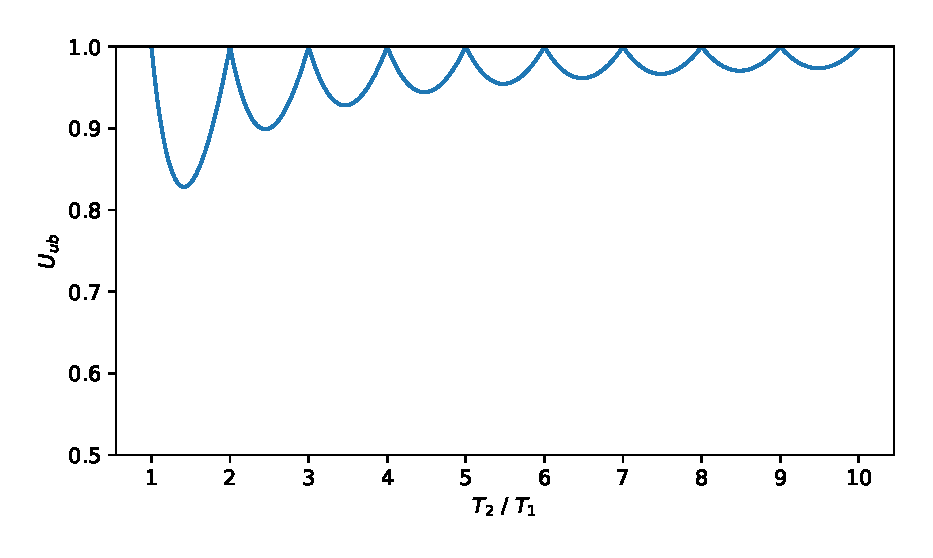
\includegraphics[width=0.7\textwidth]{figures/ub_rm_2tasks.eps}
    \caption{The upper bound on processor utilization using the Rate Monotonic algorithm, as the ratio between task periods $T_1$ and $T_2$ varies. Adapted from \textcite{buttazzo2011hard}.}
    \label{fig:ubk}
\end{figure}

The Liu-Layland schedulability test is, however, not exact -- it rejects task sets which could be executed without missing any deadlines. Better schedulability tests are given by \textcite{Bini2003}, which gives a less strict sufficient condition (improving the acceptance ratio up to $\sqrt{2}$ for a large number of tasks), and exact schedulability tests are given in \textcite{Lehoczky1989} and \textcite{Audsley1993}.

\subsection{Earliest Deadline First}
Depending on task set characteristics, Earliest Deadline First schedulability analysis can be very simple. Liu and Layland show that the upper bound on processor utilization for EDF is 1, and this turns out to be a necessary and sufficient condition if task deadlines are equal to their periods. That is, for a given task set $\Gamma$ with tasks $\tau_1, \tau_2, \ldots, \tau_m$ whose relative deadline is equal to their period, iff

\begin{equation}
    U_\Gamma = \sum_{i=1}^m \dfrac{C_i}{T_i} \le 1
\end{equation}

\noindent the task set is schedulable under EDF.

In case task deadlines are less than or equal to their periods, schedulability analysis becomes more complicated. \textcite{Baruah1990} propose the \emph{Processor Demand Criterion}, which computes the processor time demand at absolute deadlines and ensures that it does not exceed the available processor time.\\

\noindent The processor demand of a task $\tau_i$ is defined on an interval $[t_1, t_2]$ as

\begin{equation}
    g_i(t_1, t_2) = \sum_{r_{i,k} \ge t_1, d_{i,k} \le t_2} C_i
\end{equation}


\noindent i.e., the computation time of task instances falling entirely between time $t_1$ and $t_2$.\\

\noindent The processor demand for an entire task set can then be defined as

\begin{equation}
    g(t_1, t_2) = \sum_{i=1}^m g_i(t_1, t_2)
\end{equation}

\noindent and the task set is feasible if, for any interval of time, the processor demand does not exceed the available processor time.\\

\noindent This criterion is used in this work.

\section{Combining periodic and aperiodic tasks}
The scheduling algorithms discussed in the previous section have been considered in purely periodic situations only. In real systems, there may be aperiodic, non-real-time jobs that must additionally be executed, such as jobs enabling human control interfaces. We would like to execute these jobs without jeopardizing real-time task schedulability. In this section, algorithms that can handle these heterogeneous task sets are discussed.

The idea behind many of these algorithms is to compute the processor utilization of the periodic task set, and set aside the rest of the processor utilization to be used by a so-called \emph{task server}, which handles aperiodic requests. The processor utilization set aside for the server, denoted $U_s$, is often called the \emph{bandwidth} of the server.

\subsection{Background Scheduling}
The simplest way of scheduling aperiodic tasks is through \emph{Background Scheduling} - simply running them when the system would otherwise be idle. One obvious downside is the large possible aperiodic task response time; periodic tasks which could be postponed while still meeting their deadlines are instead run earlier than they have to be, delaying aperiodic tasks. For this reason, more advanced aperiodic job servers have been developed.

\subsection{Total Bandwidth Server}
The \emph{Total Bandwidth Server} is a server for aperiodic jobs which is used in conjunction with the EDF algorithm. When an aperiodic job $j_k$ enters the system, at $t = a_k$, it receives a deadline

\begin{equation}
    d_k = \max(a_k, d_{k-1}) + \frac{C_k}{U_s}
\end{equation}

where $U_s$ is the server bandwidth and $C_k$ is the job's worst-case execution time. The name of the server is reflected in the fact that the total bandwidth over a given time period is given to the job.

After this deadline is assigned, the job is scheduled by the EDF algorithm, as are the periodic tasks in the system.

\subsubsection{Optimizing TBS: deadline advancement}
Note that this deadline is pessimistic, in the sense that it could be set earlier, improving aperiodic response time, if the finishing time of $j_k$, $f_k$, is earlier than its assigned deadline. The set deadline accounts for the worst-case periodic schedule, as it only takes into account the processor utilization used by periodic tasks. In many situations, the periodic schedule is less pessimal. For instance, let us take the situation in figure~\ref{fig:tbsworstdeadline}. Here, we have periodic processor utilization $U_p = \frac{5}{6}$, and server bandwidth $U_s = \frac{1}{6}$. The deadline assigned to $j_k$, which has computation time $C_k = 2$ and arrives at $t = 2$, is therefore $d_k = 2 + \frac{C_k}{U_s} = 14$. Due to the strange (non-EDF) periodic schedule, it also finishes at $t = 14$. EDF, with deadline $d_k = 14$, produces a schedule where $j_k$ finishes at $f_k = 12$ (fig. \ref{fig:tbsedfdeadline}). Knowing this, we could set its deadline to $12$. However, if we then recompute its EDF schedule, we will find that the task finishes even earlier. This process can be repeated to find $j_k$'s earliest finishing time, $f^*_k$, which turns out to be $5$, as can be seen in figure~\ref{fig:tbsoptimaldeadline}. As you can see, the response time of $j_k$ can be greatly improved, without jeopardizing periodic tasks. The drawback is added computational complexity, due to the fact that evaluating $f^*_k$ requires (repeatedly) computing the EDF schedule up to the finishing time of $j_k$.

\begin{figure}[htpb]
    \centering
    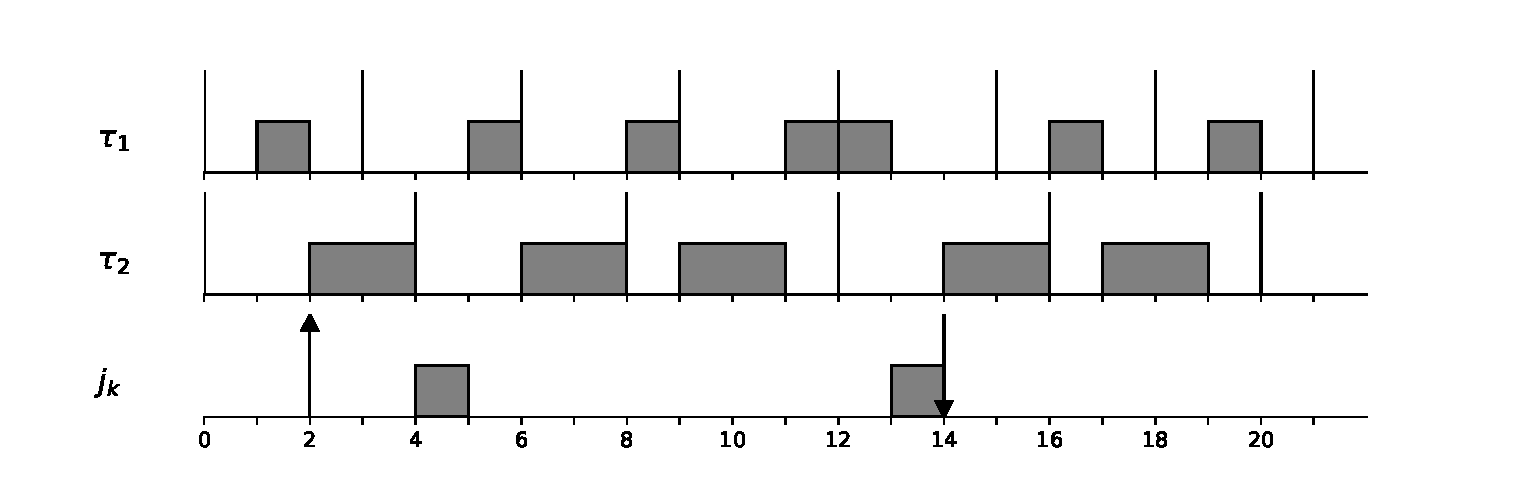
\includegraphics[width=0.85\textwidth]{figures/worstcasedeadline.eps}
    \caption{A situation where job $j_k$ finishes exactly at its deadline.}
    \label{fig:tbsworstdeadline}
\end{figure}

\begin{figure}[htpb]
    \centering
    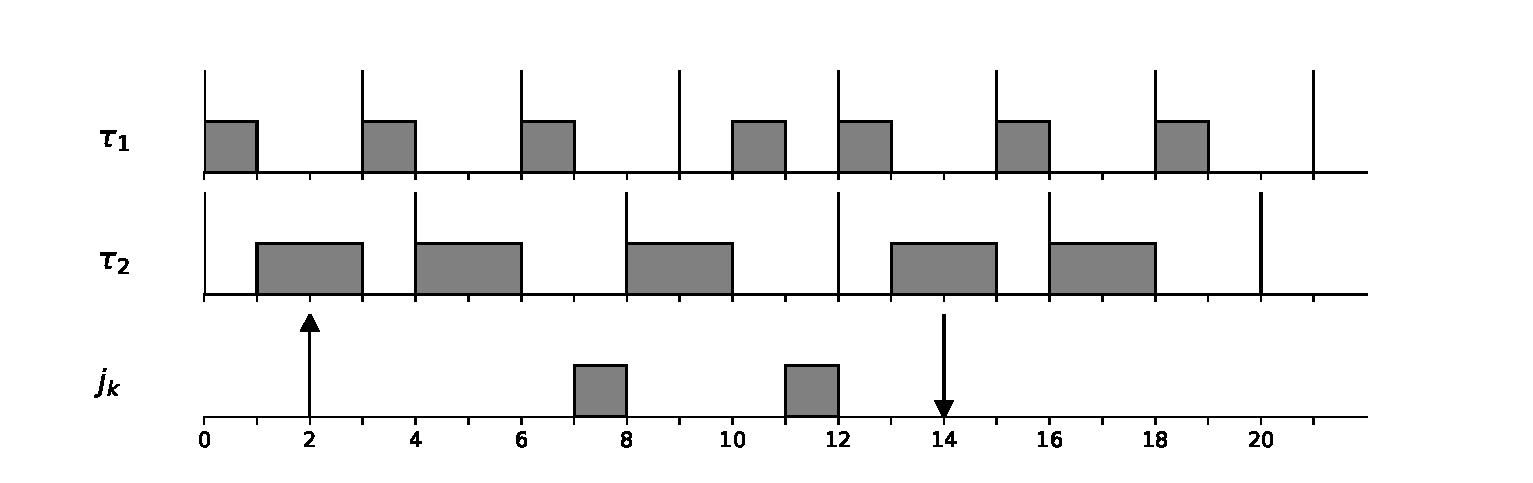
\includegraphics[width=0.85\textwidth]{figures/edfdeadline.eps}
    \caption{The situation produced by EDF, where $f_k$ = 12.}
    \label{fig:tbsedfdeadline}
\end{figure}

\begin{figure}[htpb]
    \centering
    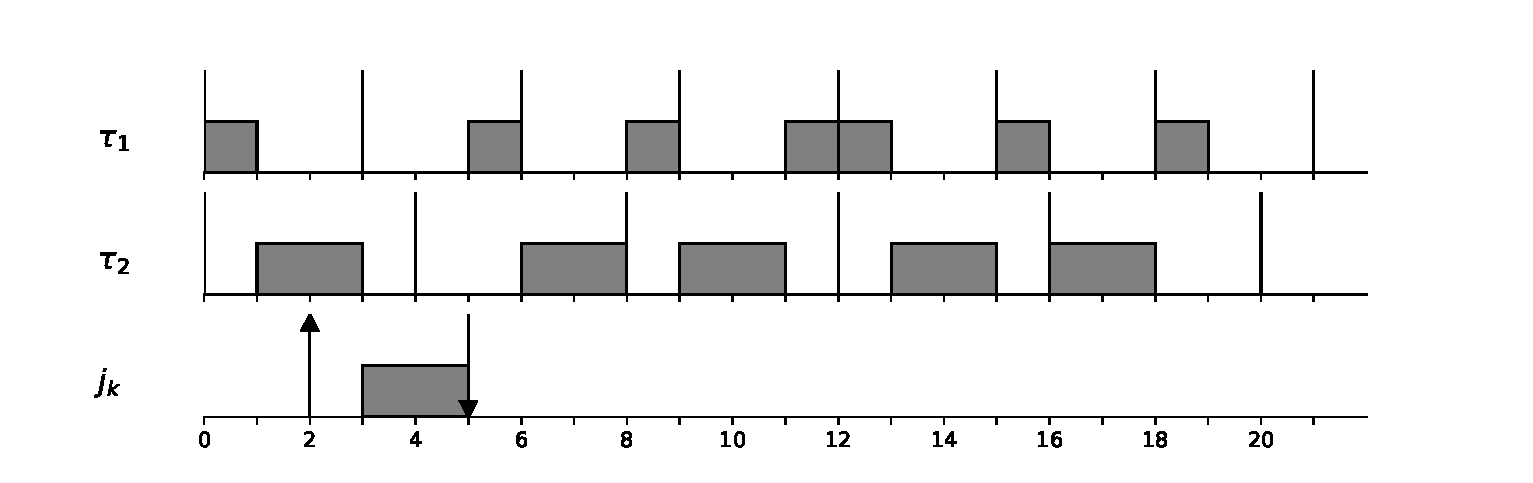
\includegraphics[width=0.8\textwidth]{figures/optimaldeadline.eps}
    \caption{The situation where $j_k$ finishes at the earliest possible time.}
    \label{fig:tbsoptimaldeadline}
\end{figure}

\section{Scheduling in \ucosiii}
Just as in many real-time operating systems, the scheduler used in \ucosiii is a generic priority-based scheduler. In these schedulers, tasks are assigned priorities and the scheduler simply runs the highest priority ready task. The priorities are assigned at task creation, but there is optional support for changing priorities at run-time. The number of priority levels is configurable at compile time.

There is optional support for round-robin scheduling. If it is enabled and multiple tasks are ready at a given priority level, each task is run for a time quantum in cyclical fashion. The length of the time quantum is configurable at task creation time.

The flexibility in the number of priority levels seems to suggest that many dynamic scheduling algorithms, such as EDF, could be built on top of the priority-based scheduler. Every additional priority level, however, brings a spatial and computational cost with it. \ucos uses a \textit{priority bitmap} (see fig.~\ref{fig:priobitmap}) to keep track of which priorities have associated ready tasks, and each priority has its own ready list. Additionally, each added priority increases the search time in the priority bitmap. This diminishes the flexibility of the scheduler, but improves the scheduling performance in the case where the number of priorities is fairly low.

Of course, the number of priority levels need only be as large as the number of tasks in the system. In this case, however, implementing an EDF scheduler becomes both more complicated and more expensive. As noted in \textcite[\S 2]{Buttazzo2005}, in the worst case, when a task priority changes, the priority of all tasks in the system may need to be remapped, an expensive operation.

For these reasons, implementing an EDF scheduler on top of the built-in scheduler is non-optimal.

\begin{figure}[ht]
    \centering
    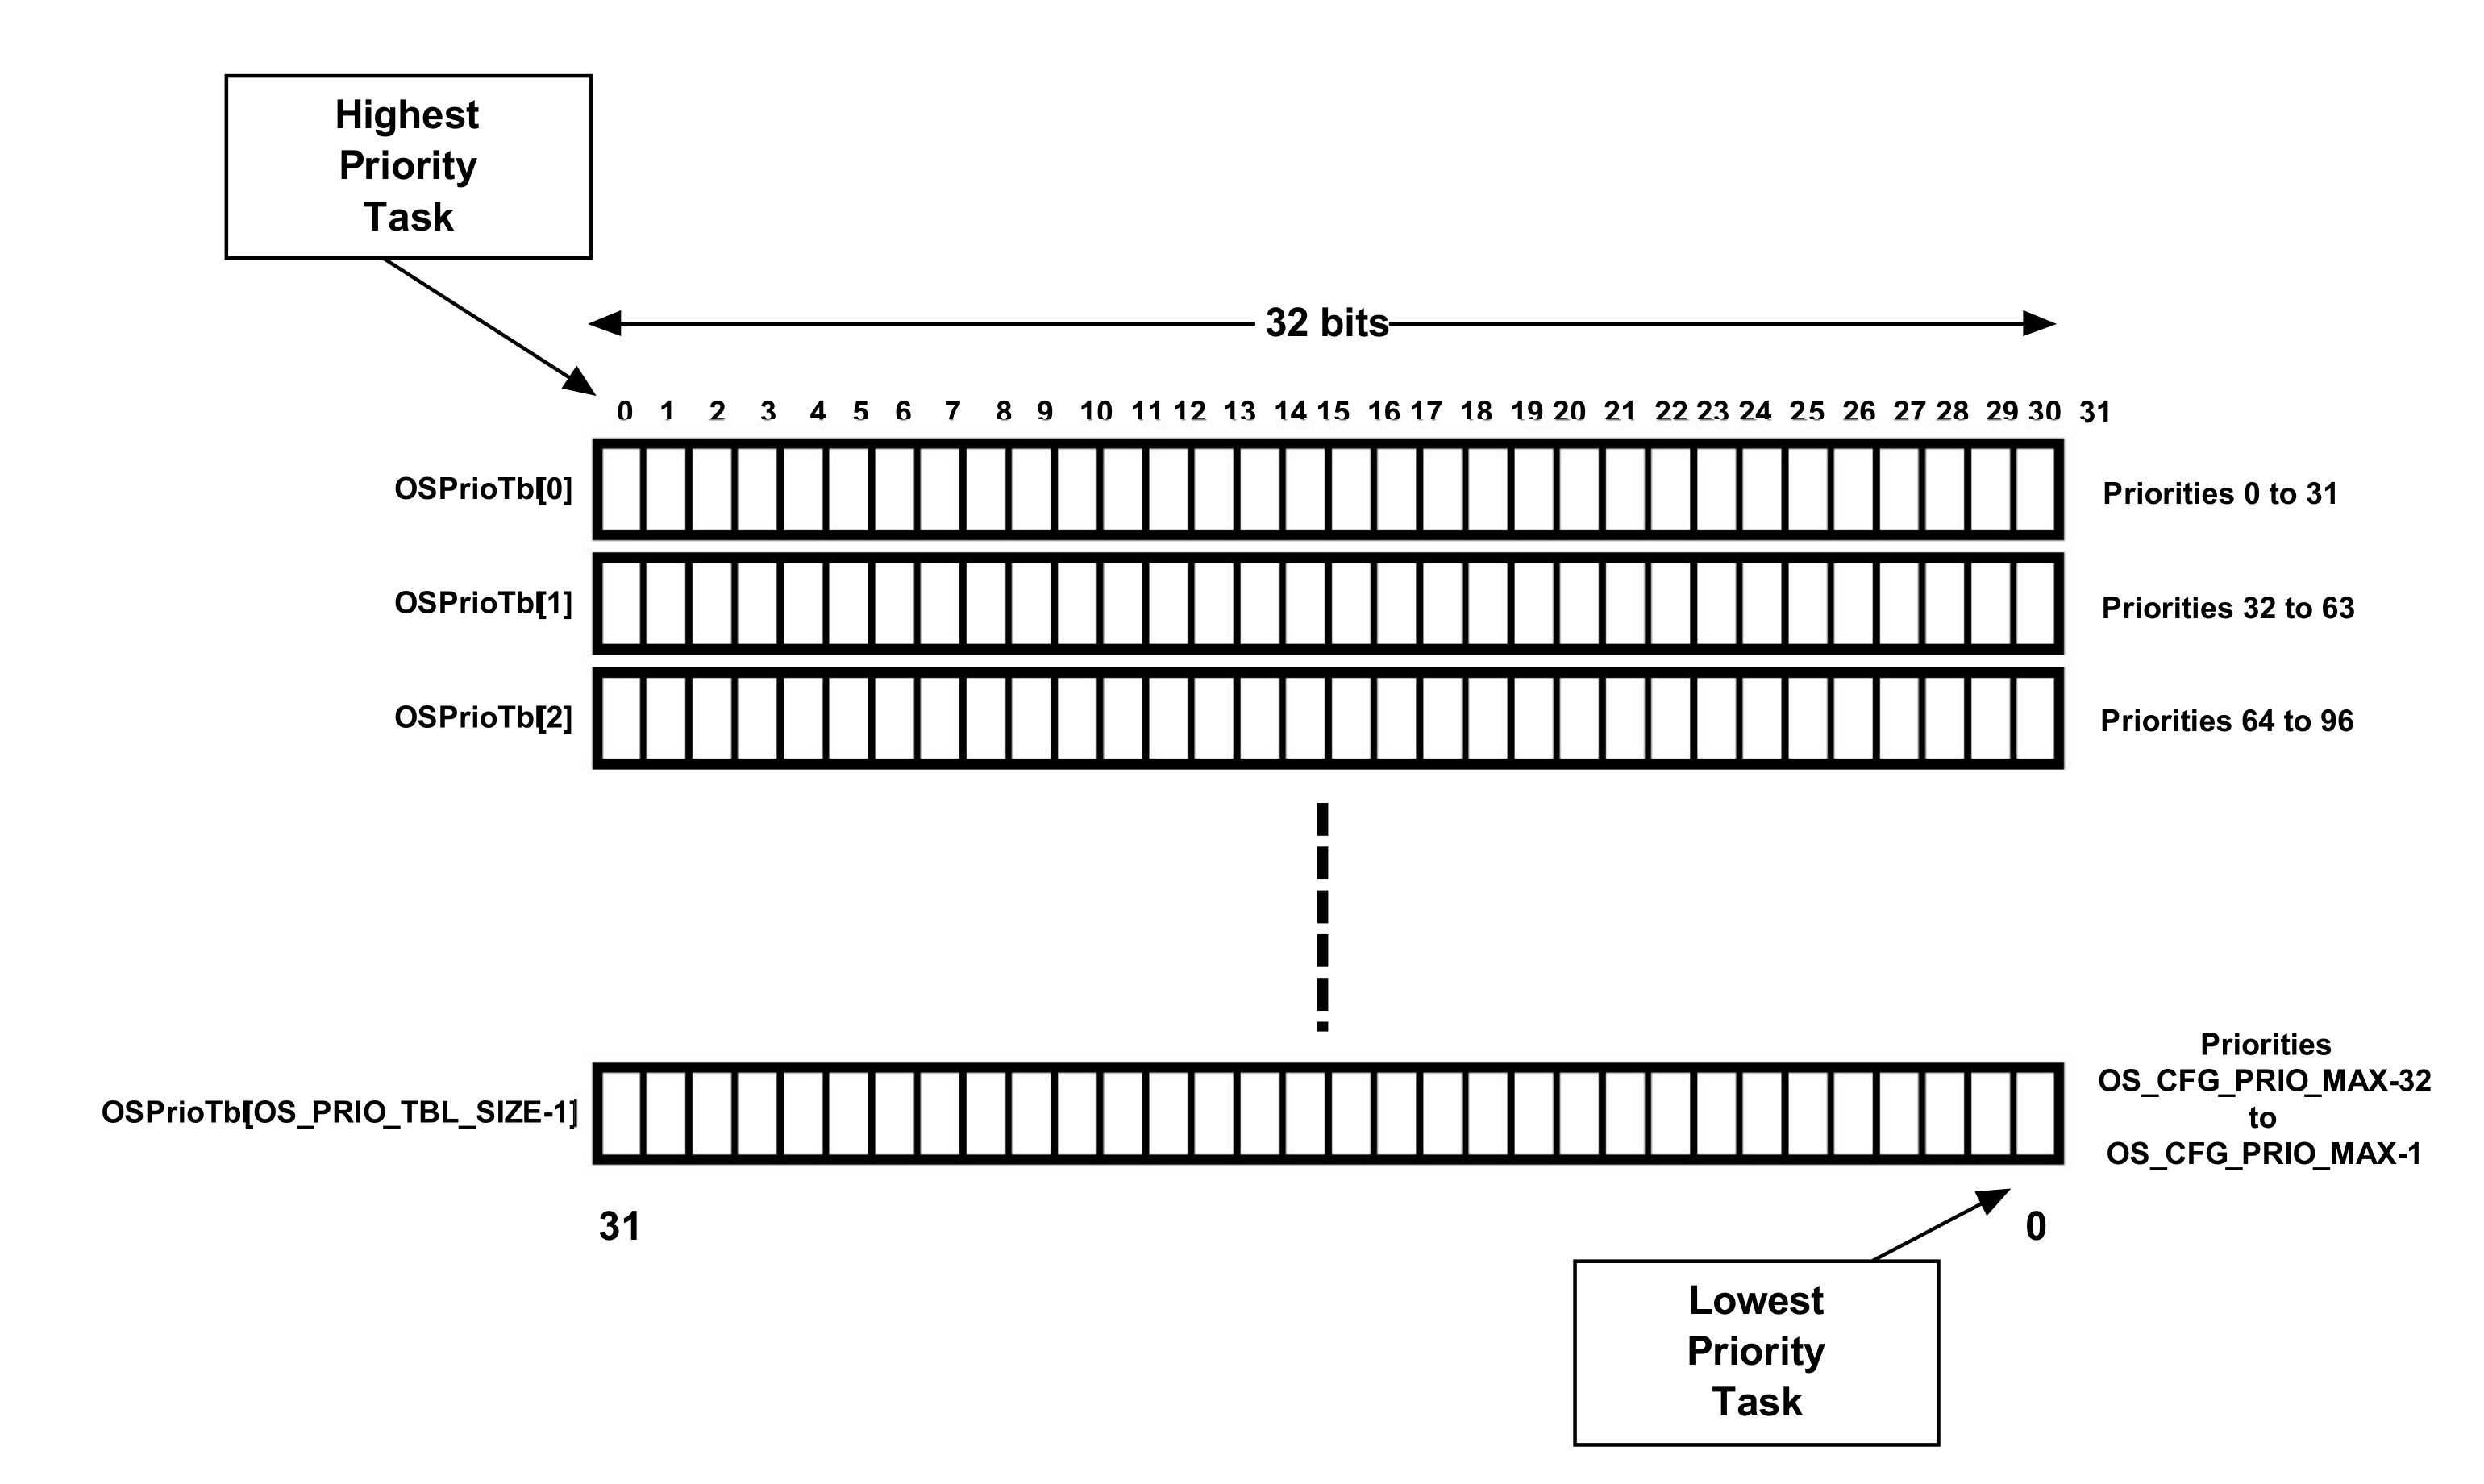
\includegraphics[width=0.8\textwidth]{figures/priobitmap.png}
    \caption{An illustration of \ucosiii's priority bitmap. Taken from the user manual, figure 6-3. If a bit is set, it indicates a ready task in the ready list of the associated priority. The highest priority task can be found quickly by using processors' `count-leading-zeros' instruction.}
    \label{fig:priobitmap}
\end{figure}


\section{Worst-case Execution Time Analysis}
Knowledge of tasks' worst-case execution times is of great importance when applying guarantee-backed scheduling. An underestimation can induce invalid guarantees, whereas overestimation will cause the system to reject task sets which may have been feasible in practice. This raises the question: how can worst-case execution times be accurately determined?

Worst-case execution time analysis is a whole discipline unto itself, with a range of analytical and measurement-based approaches. Ideally, a mix of analytical and measurement-based approaches is used, as analytical static analysis often fails to take into account run-time behavior such as caching, while a purely measurement-based approach may be limited due to the scarcity of extremely long execution times.

\subsection{Extreme Value Theory-based Worst-case Execution Time Analysis}

\textcite{hansen_et_al:wcet} detail a method of determining worst-case execution times based on a fusion of measurement-based and analytical approaches. The method makes use of extreme value theory, a branch of mathematics which is concerned with reasoning about the tails of distributions. Using extreme value theory, \citeauthor*{hansen_et_al:wcet} reason that the \emph{block maxima} of execution times are distributed according to the generalized extreme value distribution, and the distribution is used to determine a probabilistic worst-case execution time.

\subsubsection{Mathematical basis}

The Fisher-Tippett-Gnedenko theorem states that the maximum of a block of $n$ independent, identically distributed random variables $X_1, X_2, \ldots, X_n$ can only converge in distribution to one of three forms of the generalized extreme value distribution; the Gumbel distribution (in case of a light-tailed underlying distribution), the Fréchet distribution (in case of a heavy-tailed underlying distribution) or the Weibull distribution (in case of a bounded-tailed underlying distribution)\footnote{A similar concept which the reader may be familiar with is the Central Limit Theorem, which states that, under certain conditions, sample means are normally distributed.}. \citeauthor*{hansen_et_al:wcet} assume worst-case execution times are distributed according to a light-tailed distribution, leading them to assume that their block maxima are distributed according to a Gumbel distribution. This assumption is verified using chi-squared tests.

\subsubsection{Method}

\citeauthor*{hansen_et_al:wcet} use a data set of execution time traces taken from a device running the VxWorks real-time operating system. They partition the 125 minutes of per-task trace data into 15 minutes of training data and 110 minutes of validation data, excluding those tasks with less than 75,000 execution time samples.

To estimate the worst-case execution time for a given task, the task execution time samples are used to fit a Gumbel distribution, and the characteristics of the Gumbel distribution can then be used to compute a probabilistic worst-case execution time, along with a probability that this execution time is exceeded.

To fit a Gumbel distribution to the given data, the execution time samples need to be divided into blocks. The correct block size is determined by using a minimum block size of 100 samples, then estimating the best-fit Gumbel parameters for the block maxima and using a chi-squared test to evaluate how well the estimated distribution fit the block maxima. In case of a bad fit, the block size is doubled and the procedure tried again. The block size used is a trade-off; the larger the block size, the more likely the block maxima will follow a Gumbel distribution, but the smaller the number of maxima that can be used to fit the distribution.

When a good set of parameters is found, the Gumbel percent-point function $F_G^{-1}$ can be used to compute a worst-case execution time estimate. The percent-point function is the inverse of the cumulative distribution function, and is defined as

\begin{equation}\label{eq:gpp}
    F_G^{-1}(q) = \mu - \beta \log(-\log (q))   
\end{equation}

\noindent where $\mu$ and $\beta$ are the two parameters of the Gumbel distribution, and $q$ is the probability that a measured block maximum does not exceed the returned block maximum. From a probability $p_e$ that a sample exceeds the block maximum, we can compute $q$ as

\begin{equation}\label{eq:gq}
    q = (1 - p_e)^b 
\end{equation}

\noindent making $q$ the probability that none of the samples exceed the WCET value. Substituting equation~\ref{eq:gq} into equation~\ref{eq:gpp} gives us the following equation

\begin{equation}
    F_G^{-1}(p_e) = \mu - \beta \log(-\log ((1 - p_e)^b))
\end{equation}

\noindent which can be used to get a worst-case execution time estimate from an exceedance probability.

